\documentclass[12pt,a4]{article}

\usepackage[utf8]{inputenc}
\usepackage[T1]{fontenc}
\usepackage{amsmath,amsfonts}
\usepackage{graphicx}

\newcommand{\R}{{\mathbb R}}
\newcommand{\C}{{\mathbb C}}
\newcommand{\N}{{\mathbb N}}
\newcommand{\ra}{\rightarrow}
\newcommand{\lra}{\longrightarrow}
\newcommand{\ind}{{\mathbf{1}}}


\title{Inversion of the Laplace transform}
\author{Robert Sirviö\\013767589}


\begin{document}

\maketitle

\section{Introduction}

Let $f:[0,\infty)\rightarrow \R$. The Laplace transform $F$ of $f$ is defined by
\begin{equation}\label{laplace}
 F(s) = \int_0^\infty e^{-st}f(t)dt,\quad s\in\C ,
\end{equation}
provided that the integral converges.     
\newline


The Laplace transformations can be very useful in the solution of partial differential equations. A basic class of partial differential equations is applicable to a wide range of problems, which is why the Laplace transformations are used frequently in e.g. system modelling, electrical circuit analysis and in digital signal processing.(\cite{transforms} ch.5.7)
\newline 

The direct problem is to determine $F$ for a given function $f$ according to (\ref{laplace}). The inverse problem is: {\em given a Laplace transform $F$, find the corresponding function $f$.} Our goal in this study is to solve the inverse problem of the Laplace transformation of a given indicator function using truncated singular value decomposition (denoted truncated SVD). We also justify and reason on the usage of truncated SVD by illustrating the ill-posedness of the inversion of the Laplace transformation.



\section{Materials and Methods}\label{sec:methods}

\subsection{The matrix model}\label{matrixModel}

Assume we know the values of $F$ at these real-valued points:
$$
 0<s_1<s_2<\ldots <s_n<\infty.
$$ 
Then we may approximate the integral in (\ref{laplace}) for example with the trapezoidal rule as
\begin{equation} \label{laptrap}
\begin{split}
 \int_0^\infty e^{-st}f(t)dt\, \approx\, \frac{t_k}{k} & \left( \frac{1}{2}e^{-st_1}f(t_1)+e^{-st_2}f(t_2)+e^{-st_3}f(t_3)+\ldots\right.\\   &\ \ \left. +e^{-st_{k-1}}f(t_{k-1})+\frac{1}{2}e^{-st_k}f(t_k)\right) ,
\end{split}
\end{equation}
where vector $t=[t_1\ t_2\ \ldots\ t_k]^T\in\R^k$, $0\leq t_1<t_2<\ldots <t_k$, contains the points at which the unknown function $f$ will be evaluated. By denoting $f_\ell=f(t_\ell), \ \ell=1,\ldots ,k$, and $m_j=F(s_j),\ j=1,\ldots ,n$, and using \eqref{laptrap}, we get a linear model of the form 
\begin{equation}\label{linearModel}
m=Af+\varepsilon
\end{equation}
with
\begin{equation}\label{LaplaceA} 
A = \frac{t_k}{k}\begin{bmatrix} \frac{1}{2}e^{-s_1t_1} & e^{-s_1t_2} & e^{-s_1t_3} & \ldots & e^{-s_1t_{k-1}} & \frac{1}{2}e^{-s_1t_k} \\
                       \frac{1}{2}e^{-s_2t_1} & e^{-s_2t_2} & e^{-s_2t_3} & \ldots & e^{-s_2t_{k-1}} & \frac{1}{2}e^{-s_2t_k} \\
                       \vdots & & & & & \vdots \\
                       \frac{1}{2}e^{-s_nt_1} & e^{-s_nt_2} & e^{-s_nt_3} & \ldots & e^{-s_nt_{k-1}} & \frac{1}{2}e^{-s_nt_k} \end{bmatrix}.
\end{equation}


\subsection{The inversion method}


\subsubsection{Singular value decomposition (SVD)}\label{sec:SVDsec}
It is considered generally known that any matrix  $A \in \R^{m \times n}$ can be written as

\begin{equation}\label{SVD}
A = UDV^T,
\end{equation}
where $U \in \R^{m \times m}$ and $V \in \R^{n \times n}$ are orthogonal and $D \in \R^{m \times n}$ is a diagonal matrix. \eqref{SVD} is known as the \emph{singular value decomposition} (SVD) of $A$. The diagonal entries $d_{i,i} \in D$, $i = 1, \ldots ,\min\{m,n\}$ are known as the \emph{singular values} of $A$, which satisfy the condition

\begin{equation*}
d_{1,1} \geq d_{2,2} \geq \ldots \geq d_{\min\{m,n\},\min\{m,n\}} \geq 0.
\end{equation*} 
We define 

\begin{equation}\label{pinv}
A^+ = VD^+U^T
\end{equation}
where $D^+ \in \R^{n \times m}$ is a diagonal matrix with diagonal entries 

\begin{equation*}
d^+_{i,i} = 
\begin{cases}
    \frac{1}{d_{i,i}}, & d_{i,i} \neq 0 \\
    0, & d_{i,i} = 0
\end{cases}
,\quad \text{where } d_{i,i} \in D \text{ and } \,i = 1, \ldots ,\min\{m,n\},
\end{equation*}
It can be proven that the minimum norm solution of a matrix equation $Af = m$, where $f,m \in R^{n \times 1}$, is obtained from $A^+m$ where $A^+$ is defined as in \eqref{pinv} (\cite{samu} p.54). This can then naturally be applied to \eqref{linearModel} yielding $f = A^+m - A^+\varepsilon$ (in the least norm sense), and especially 
$f = A^+m$ when $\varepsilon = 0_{n \times 1}$. We see that 

\begin{align*}
||A^+||_2 = ||VD^+U^T||_2 &\leq  ||V||_2||D^+||_2||U^T||_2 = ||D^+||_2\\
&=\sqrt{\sum_{k=1}^{\min\{m,n\}}\left( d^+_{k,k} \right)^2},
\end{align*}
and because

\begin{equation*}
||A^+ \varepsilon||_2 \leq ||A^+||_2||\varepsilon||_2
\end{equation*}
we see that very low-valued diagonal entries in $D$ might amplify the error quite much (see also \cite{samu} p.50). To counter this we introduce the truncated SVD method.

\subsubsection{Truncated SVD}\label{sec:truncSVD}
For any $\alpha > 0$ we define the \emph{truncated} SVD by 
\begin{equation}\label{truncSVD}
A^+_\alpha = V D^+_\alpha U^T
\end{equation}
where $A$, $U$, $D$ and $V$ are defined as in section \ref{sec:SVDsec}, and 
\begin{equation*}
(d^+_\alpha)_{i,i} = 
\begin{cases}
    \frac{1}{d_{i,i}}, & 
    d_{i,i} \in \left\{d_{i,i} \in D:d_{i,i} > \alpha \right\} \\
    0, & \text{otherwise}
\end{cases}
,\quad\quad i = 1, \ldots, \min\{m,n\}
\end{equation*}
That is, we exclude the singular value entries from the diagonal matrix $D$ that fall below a certain threshold. This is used in order to counter the amplifying effect of the error discussed in \ref{sec:SVDsec}.


\subsection{The basis and materials}\label{sec:basis}

In our study we specify our target function to be defined as an indicator function:
\begin{equation}\label{fdef}
f:[0,\infty) \lra \R, \quad f = \ind_{[0,1]},
\end{equation}

that is

\begin{equation*}
f(x) = \ind_{[0,1]}(x)=
\begin{cases}
    1, \quad x \in [0,1]\\
    0, \quad \text{otherwise}.
\end{cases}
\end{equation*}
We will construct synthetic data by defining a partition of size $n$ over a predefined domain $[0,a]$, $a < \infty$ and then map the partition over $F$ and finally add some noise to the data. More explicitly, we have a partition $0=s_0 < s_1 < \ldots <s_n = a$ from which we get the data 
$\{F(s_k) + \varepsilon_k\}_{k = 0, \ldots, n}$, where $\varepsilon_k$ denotes the noise-factor for which $\varepsilon_k \in \R \quad \forall k=0 \ldots n$. We allow equality to zero for the noise to demonstrate the inverse crime. Now, because of the definition in \eqref{fdef}, we see that for all $s \neq 0$  

\begin{equation*}
F(s) = \int_0^\infty e^{-st}f(t)dt 
     = \int_0^\infty e^{-st}\ind_{[0,1]}(t)dt
     = \int_0^1 e^{-st}dt
     = -\frac{1}{s}\left(e^{-s} - 1\right)
\end{equation*}

and

\begin{equation*}
F(0) = \int_0^1 e^{0}dt = 1,
\end{equation*}
which makes the evaluation of the Laplace transform (and thus also the computation of the data) in our case very straight-forward and computationally efficient. This data will then be used to construct the linear model defined by \eqref{linearModel}, which we then attempt solve and reconstruct our target indicator function with truncated SVD.

\section{Results}\label{sec:results}

As section \ref{sec:basis} implies, the Laplace transformation of the predefined indicator function will reduce to an exponential function, which will also be the basis of the data generation. Figure \ref{fig:laplacePlot} illustrates the Laplace transformation and the data generation with 
$\varepsilon_k \sim U(-0.01,0.01)$ for all $k$.

\begin{figure}[h]
\begin{picture}(250,190)
\put(-30,0){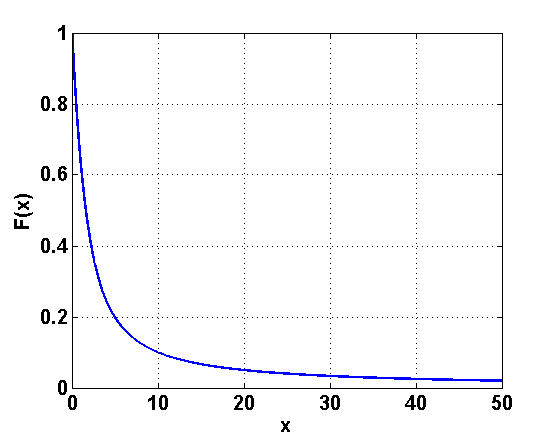
\includegraphics[height=7cm, width=8cm]{pics/lap_range-0-50.png}}
\put(180,0){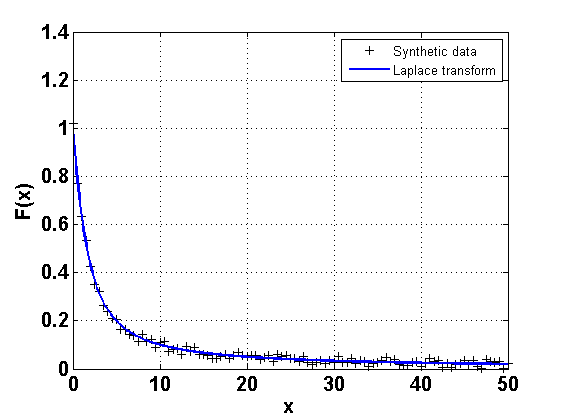
\includegraphics[height=7cm, width=8cm]{pics/synthetic_data_plot.png}}
\end{picture}
\caption{Graph of the Laplace transform $F$ of $f = \ind_{[0,1]}$ and synthetic data generation}
\label{fig:laplacePlot}
\end{figure}

The coefficient matrix, defined in \eqref{LaplaceA}, of the linear system defined in \eqref{linearModel} is constructed using the trapezoidal formula suggested in \eqref{laptrap}. A coefficient matrix of this kind is illustrated in figure \ref{fig:coeffMatPlot}, where
\begin{equation*}
\max\{a_{i,j}: a_{i,j} \in A\} = 0.02 \text{, and }
\min\{a_{i,j}: a_{i,j} \in A\} \approx 8 \cdot 10^{-42}.
\end{equation*}
and with a partition of size 150 for both $s$ values over the range $[0,30]$ and $t$ values over the range $[0,3]$.

\begin{picture}(150,115)\label{fig:coeffMatPlot}
\put(45,0){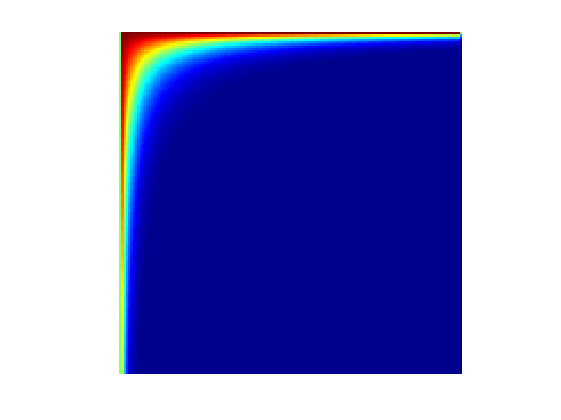
\includegraphics[height=6cm]{pics/coefmat_sRange-0-30_tRange-0-3_points-150.png}}
\end{picture}


Singular value computations were done for coefficient matrices with partitions over the range $[0,1]$, where

\begin{equation*}
t_k = \frac{k}{n} \text{, } s_k = \frac{k}{n} \text{ where } 
n = 10,100 \text{ for all } k = 0, \ldots , n.
\end{equation*}
Results of these computations are illustrated in figure \ref{fig:svdPLot}, where both of the plots have a logarithmically scaled y-axis.

\begin{picture}(200,240)\label{fig:svdPLot}
\put(-40,0){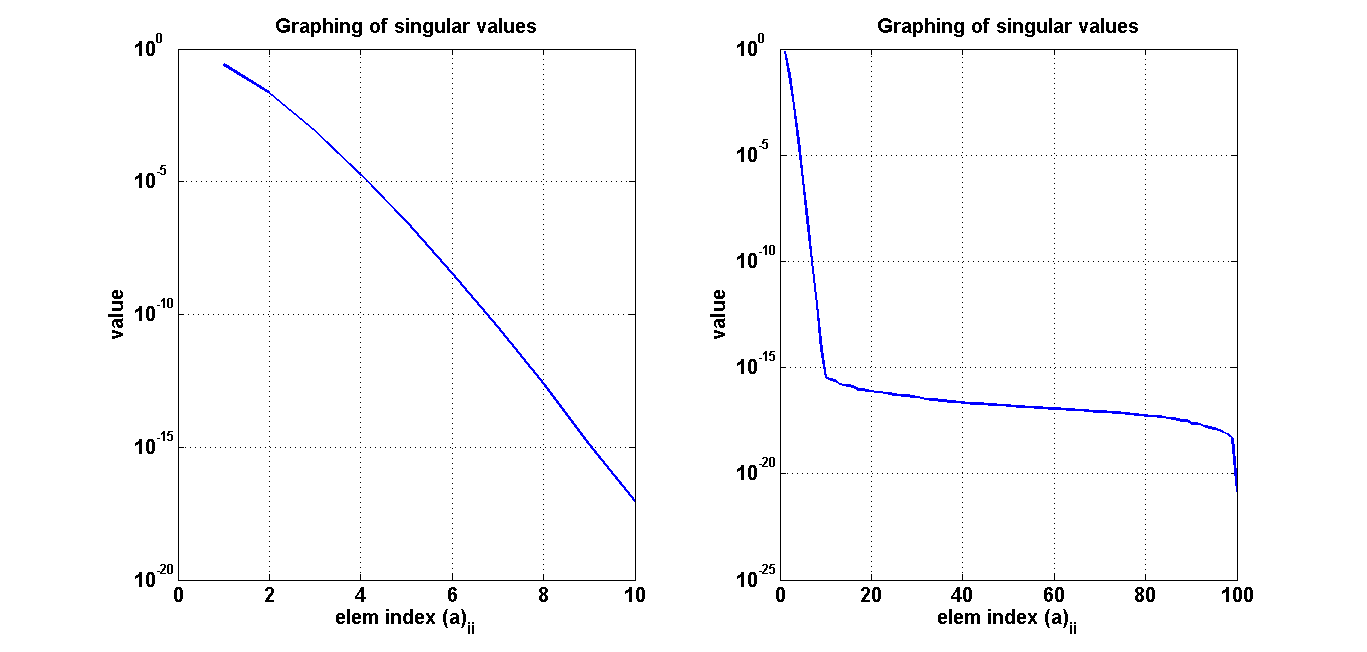
\includegraphics[height=7.5cm]{pics/svd_range-0-1_points-10-100.png}}
\end{picture}

Finally reconstructions were computed using the truncated SVD method defined in section \ref{sec:truncSVD} with different (uniformly distributed) error vectors. Detailed info of computations  are included beneath each figure. The \emph{Tol} value in the plots indicate the threshold values ($\alpha$ values) of truncated SVD and the \emph{error} value indicates the relative error of the reconstruction.

\begin{picture}(200,190)\label{fig:recPlot1}
\put(0,30){\includegraphics[height=7cm]{pics/rec_with_no_noise.png}}
\put(0,30){Figure 4: s range: $[0,60]$, partition size of s: 1000, partition size of t: 1000,}
\put(0,15){$\varepsilon_k = 0$ for all $k$}
\end{picture}

\begin{picture}(200,340)\label{fig:recPlot2}
\put(-160,0){\includegraphics[height=12cm]{pics/recPlot_error-1e-8_sRange-60_sPoints-30_tPoints-4000.png}}
\put(0,0){Figure 5: s range: $[0,60]$, partition size of s: 30, partition size of t: 4000,} 
\put(0,-17){$\varepsilon_k \sim U(10^{-8}, 10^{-8})$ for all $k$}
\end{picture}

\begin{picture}(200,350)\label{fig:recPlot3}
\put(-160,0){\includegraphics[height=12cm]{pics/recPlot_error-1e-6_sRange-60_sPoints-30_tPoints-4000.png}}
\put(0,0){Figure 6: s range: $[0,60]$, partition size of s: 30, partition size of t: 4000,} 
\put(0,-17){$\varepsilon_k \sim U(10^{-6}, 10^{-6})$ for all $k$}
\end{picture}

\newpage

\section{Discussion}\label{sec:discussion}

As the graphing of the singular values in figure 3 indicates, one can see that the singular values of the coefficient matrix decreases rapidly, which in turn indicates ill-posedness of the inversion (for an attentive reader this might be already clear from the second figure illustrating the coefficient matrix, as it shows properties that closely resemble the ones of the very ill-conditioned Hilbert's matrix). This essentially justifies our use of the truncated SVD method for computing the inversion versus the naïve method as indicated by figures 4-6; even though we get a very good reconstruction with the naïve method from data without error (see figure 4), we can clearly see from figures 5 and 6 that the reconstructions fall apart when we include singular values lower than $10^{-14}$ and $10^{-10}$. We can, however, conclude from figures 5 and 6 that the truncated SVD method produces reconstructions with acceptable relative error range with sufficiently large $\alpha$ values.
\\

Another thing worth mentioning is the use of uniformly distributed error vectors in the data generation; although it might be considered unorthodox or even unrealistic to not use error samples from the normal distribution, the benefit of using samples from the uniform distribution is that we are then able to bound the error factor and thus construct results that are easier to reproduce.


\newpage
\begin{thebibliography}{9}
\bibitem{samu}
	Mueller, Jennifer L. \& Siltanen Samuli \emph{Linear and Nonlinear Inverse Problems with Practical Applications}.\\
	SIAM, 1:st edition, 2012

\bibitem{transforms}
    Poularikas, Alexander D. \emph{Transforms and Applications Handbook}.\\
    CRC Press, 3:rd edition, 2009 

\end{thebibliography}

\end{document}



